\documentclass[aspectratio=169]{../latex_main/tntbeamer}  % you can pass all options of the beamer class, e.g., 'handout' or 'aspectratio=43'
\usepackage{dsfont}
\usepackage{bm}
\usepackage[english]{babel}
\usepackage[T1]{fontenc}
%\usepackage[utf8]{inputenc}
\usepackage{graphicx}
\graphicspath{ {./figures/} }
\usepackage{algorithm}
\usepackage[ruled,vlined,algo2e,linesnumbered]{algorithm2e}
\usepackage{hyperref}
\usepackage{booktabs}
\usepackage{mathtools}

\usepackage{amsmath,amssymb}

\DeclareMathOperator*{\argmax}{arg\,max}
\DeclareMathOperator*{\argmin}{arg\,min}

\usepackage{amsbsy}
\newcommand{\vect}[1]{\bm{#1}}
%\newcommand{\vect}[1]{\boldsymbol{#1}}

\usepackage{pgfplots}
\pgfplotsset{compat=1.16}
\usepackage{tikz}
\usetikzlibrary{trees} 
\usetikzlibrary{shapes.geometric}
\usetikzlibrary{positioning,shapes,shadows,arrows,calc,mindmap}
\usetikzlibrary{positioning,fadings,through}
\usetikzlibrary{decorations.pathreplacing}
\usetikzlibrary{intersections}
\pgfdeclarelayer{background}
\pgfdeclarelayer{foreground}
\pgfsetlayers{background,main,foreground}
\tikzstyle{activity}=[rectangle, draw=black, rounded corners, text centered, text width=8em]
\tikzstyle{data}=[rectangle, draw=black, text centered, text width=8em]
\tikzstyle{myarrow}=[->, thick, draw=black]

% Define the layers to draw the diagram
\pgfdeclarelayer{background}
\pgfdeclarelayer{foreground}
\pgfsetlayers{background,main,foreground}

% Requires XeLaTeX or LuaLaTeX
%\usepackage{unicode-math}

\usepackage{fontspec}
%\setsansfont{Arial}
\setsansfont{RotisSansSerifStd}[ 
Path=../latex_main/fonts/,
Extension = .otf,
UprightFont = *-Regular,  % or *-Light
BoldFont = *-ExtraBold,  % or *-Bold
ItalicFont = *-Italic
]
\setmonofont{Cascadia Mono}[
Scale=0.8
]

% scale factor adapted; mathrm font added (Benjamin Spitschan @TNT, 2021-06-01)
%\setmathfont[Scale=1.05]{Libertinus Math}
%\setmathrm[Scale=1.05]{Libertinus Math}

% other available math fonts are (not exhaustive)
% Latin Modern Math
% XITS Math
% Libertinus Math
% Asana Math
% Fira Math
% TeX Gyre Pagella Math
% TeX Gyre Bonum Math
% TeX Gyre Schola Math
% TeX Gyre Termes Math

% Literature References
\newcommand{\lit}[2]{\href{#2}{\footnotesize\color{black!60}[#1]}}

%%% Beamer Customization
%----------------------------------------------------------------------
% (Don't) Show sections in frame header. Options: 'sections', 'sections light', empty
\setbeamertemplate{headline}{empty}

% Add header logo for normal frames
\setheaderimage{
	% 
\includegraphics[height=\logoheight]{figures/TNT_darkv4.pdf}
	
\includegraphics[height=\logoheight]{../latex_main/figures/luh_logo_rgb_0_80_155.pdf}
	% 
\includegraphics[height=\logoheight]{figures/logo_tntluh.pdf}
}

% Header logo for title page
\settitleheaderimage{
	% 
\includegraphics[height=\logoheight]{figures/TNT_darkv4.pdf}
	
\includegraphics[height=\logoheight]{../latex_main/figures/luh_logo_rgb_0_80_155.pdf}
	% 
\includegraphics[height=\logoheight]{figures/logo_tntluh.pdf}
}

% Title page: tntdefault 
\setbeamertemplate{title page}[tntdefault]  % or luhstyle
% Add optional title image here
%\addtitlepageimagedefault{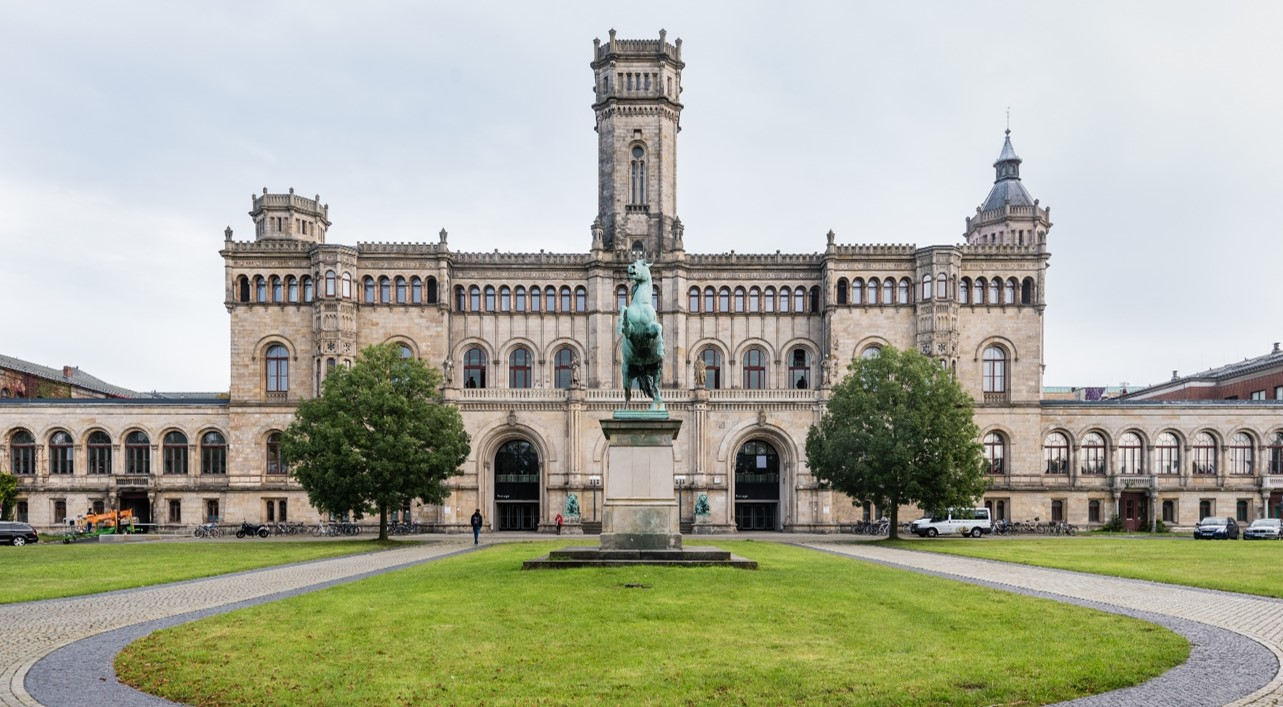
\includegraphics[width=0.65\textwidth]{figures/luh_default_presentation_title_image.jpg}}

% Title page: luhstyle
% \setbeamertemplate{title page}[luhstyle]
% % Add optional title image here
% \addtitlepageimage{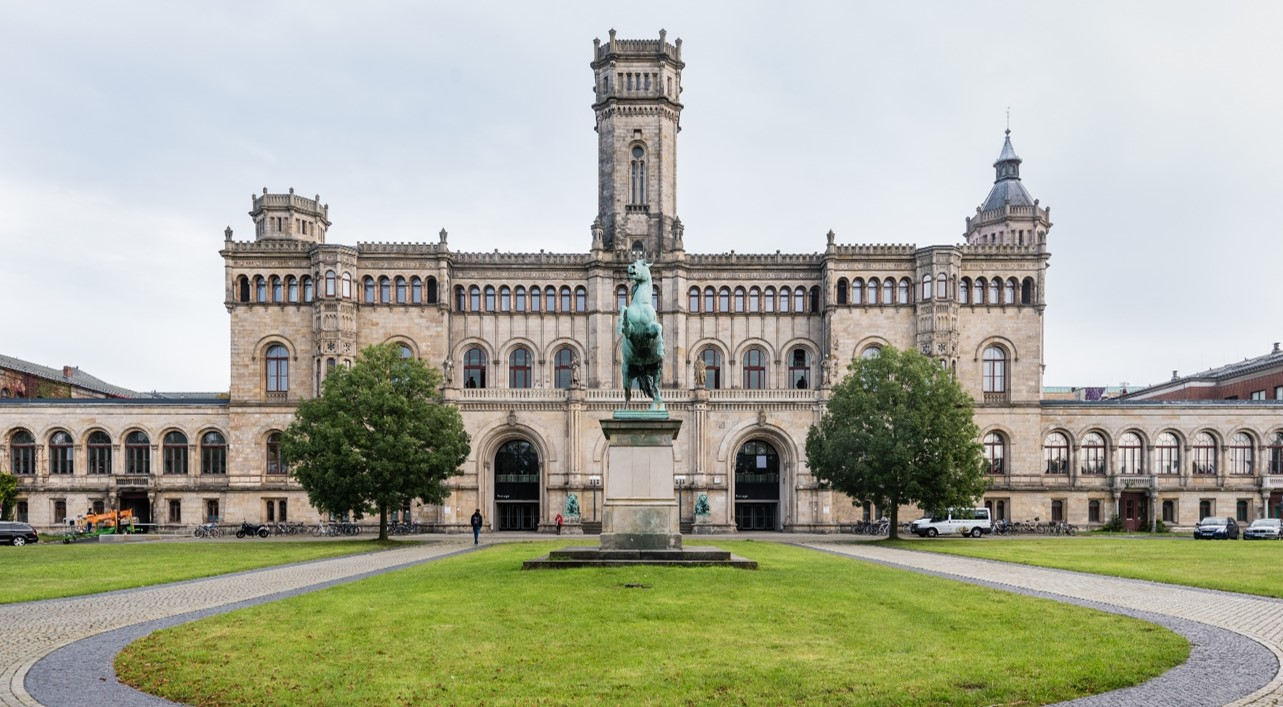
\includegraphics[width=0.75\textwidth]{figures/luh_default_presentation_title_image.jpg}}

\author[Abedjan \& Lindauer]{Ziawasch Abedjan \& Marius Lindauer\\[1em]
	
\includegraphics[height=\logoheight]{../latex_main/figures/luh_logo_rgb_0_80_155.pdf}\qquad
	
\includegraphics[height=\logoheight]{../latex_main/figures/DBIS_Kurzlogo.png}\qquad

\includegraphics[height=\logoheight]{../latex_main/figures/TNT_darkv4}\qquad

\includegraphics[height=\logoheight]{../latex_main/figures/L3S.jpg}	}
\date{Summer Term 2022; \hspace{0.5em} {
\includegraphics[height=1.5em]{../latex_main/figures/Cc-by-nc-sa_icon.svg.png}}; based on \href{https://ds100.org/fa21/}{[DS100]}
}


%%% Custom Packages
%----------------------------------------------------------------------
% Create dummy content
\usepackage{blindtext}

% Adds a frame with the current page layout. Just call \layout inside of a frame.
\usepackage{layout}


%%% Macros
%\renewcommand{\vec}[1]{\mathbf{#1}}
% \usepackage{bm}
%\let\vecb\bm

\title[DL: Transformers]{DS: Deep Learning}
\subtitle{Transformers}

\date{\hspace{0.5em} {
\includegraphics[height=1.5em]{../latex_main/figures/Cc-by-nc-sa_icon.svg.png}} inspired by \href{https://www.youtube.com/watch?v=bQ5BoolX9Ag}{StatQuest by Joshua Starmer}}

\graphicspath{ {./figure/} }
%\institute{}


\begin{document}
	
	\maketitle


        %%%%%%%%%%%%%%%%%%%%%%%%%%%%%%%%%%%%%%%%%%%%%%%%%%%%%%%%%%%%%%
        \begin{frame}{Tranformers [\href{https://arxiv.org/pdf/1706.03762}{Vaswani et al. 2017}]}

        \begin{columns}

        \begin{column}{0.5\textwidth}

            \begin{itemize}
                \item Transformers are state of the art in many applications these days
                \item They allow to processing of huge amounts of data efficiently
                \item Key concepts include
                \begin{itemize}
                    \item They understand the context
                    \item They attend to the most important context
                    \item They process all at once (e.g., input of an entire paragraph of text instead of word by word)
                    \item Let's understand the main concepts step by step
                \end{itemize}
            \end{itemize}

        \end{column}

        \begin{column}{0.5\textwidth}

        \centering
        \vspace*{-2em}
        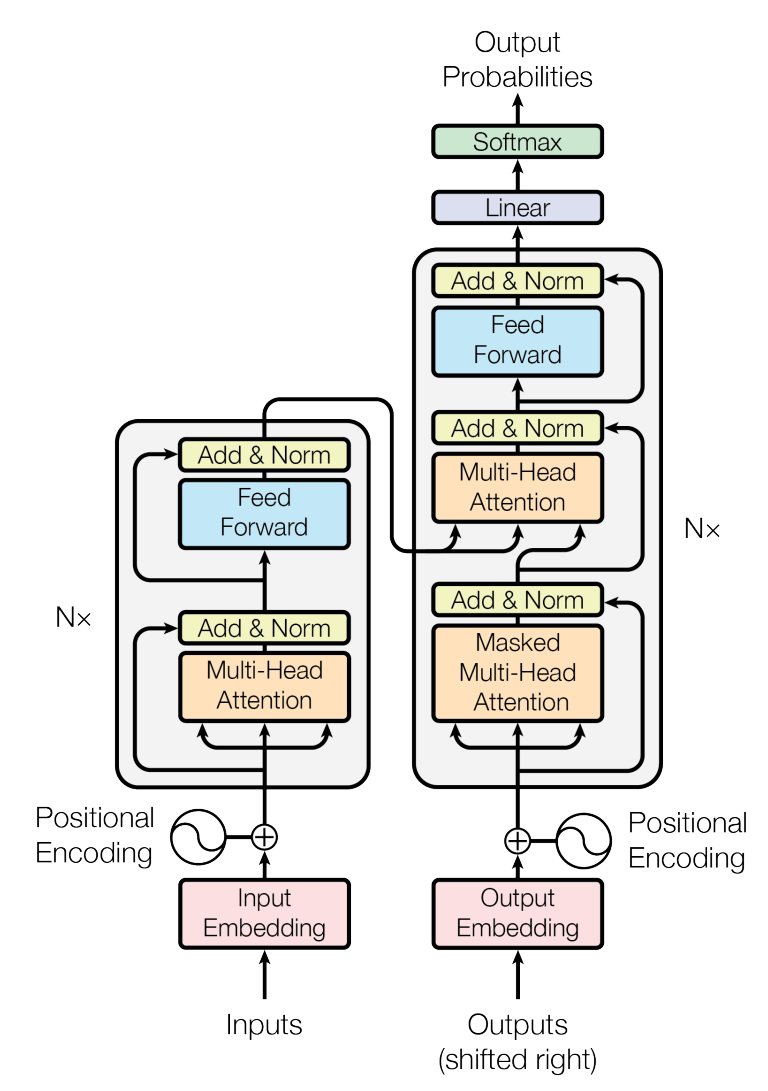
\includegraphics[width=0.6\textwidth]{figures/transformer.png}\\
        Credits: [\href{https://arxiv.org/pdf/1706.03762}{Vaswani et al. 2017}]

        \end{column}
            
        \end{columns}
        
        \end{frame}

        %%%%%%%%%%%%%%%%%%%%%%%%%%%%%%%%%%%%%%%%%%%%%%%%%%%%%%%%%%%%%%
        \begin{frame}{Exemplary Chat I}

            \centering
            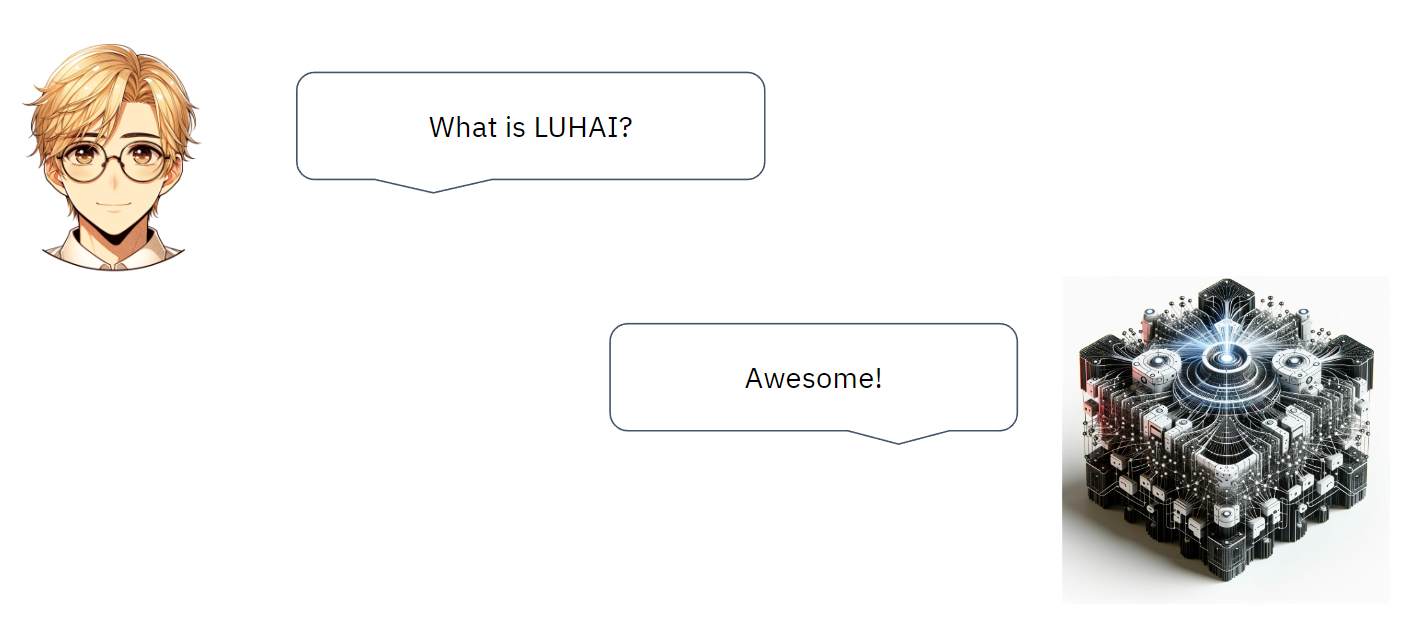
\includegraphics[width=1\linewidth]{075_deep_learning/figures/transformer1.png}
        
        \end{frame}

        %%%%%%%%%%%%%%%%%%%%%%%%%%%%%%%%%%%%%%%%%%%%%%%%%%%%%%%%%%%%%%
        \begin{frame}{Step 1: Word Embedding}

            \begin{itemize}
                \item Computers cannot directly work on words $\leadsto$ numbers are better
                \item Let's translate all the words of a vocabulary into a vector
                \begin{itemize}
                    \item in addition <EOS> or <SOS (end/start of sequence)
                \end{itemize}
            \end{itemize}

            \centering
            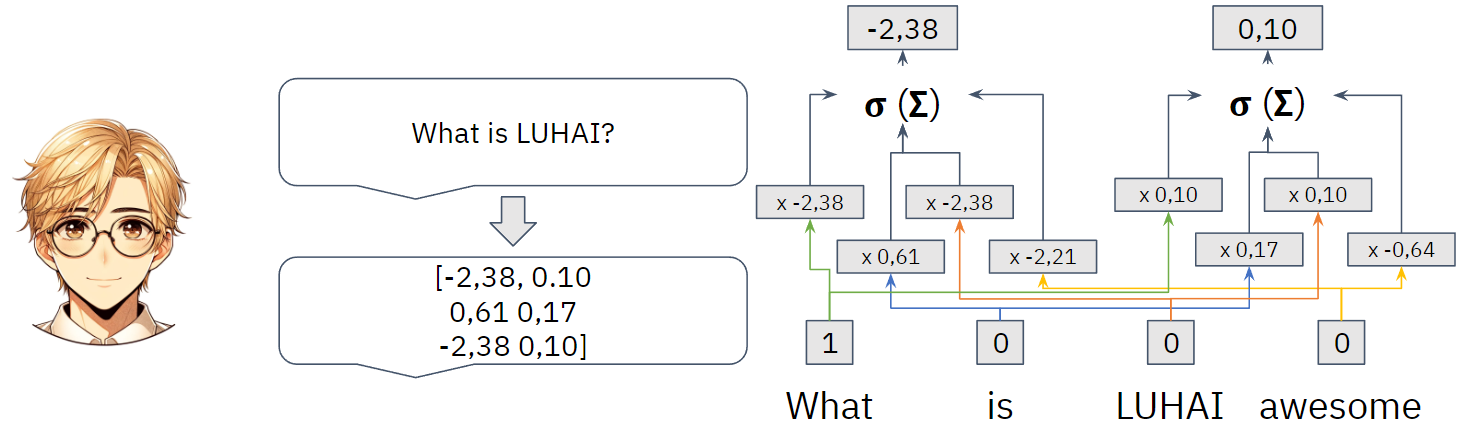
\includegraphics[width=1\linewidth]{075_deep_learning/figures/transformer2.png}
        
        \end{frame}

        %%%%%%%%%%%%%%%%%%%%%%%%%%%%%%%%%%%%%%%%%%%%%%%%%%%%%%%%%%%%%%
        \begin{frame}{Exemplary Chat II}

            \begin{itemize}
                \item Order matters!
            \end{itemize}

            \centering
            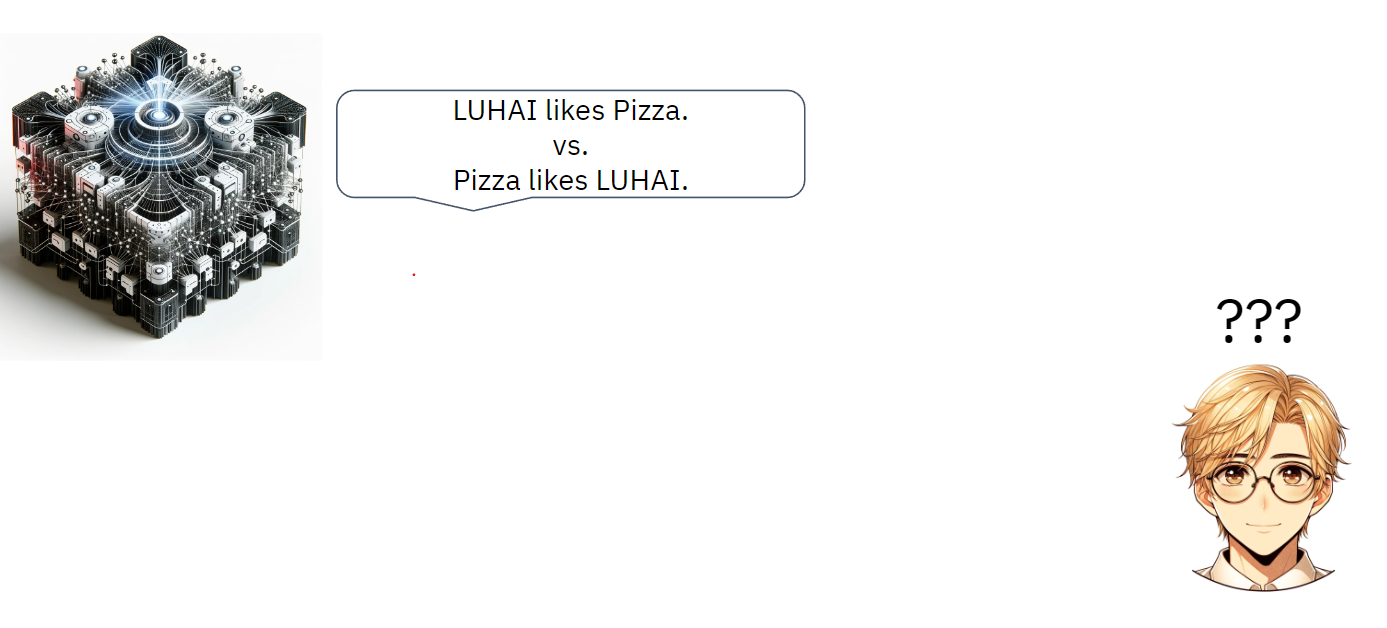
\includegraphics[width=0.9\linewidth]{075_deep_learning/figures/transformer3.png}
        
        \end{frame}

        %%%%%%%%%%%%%%%%%%%%%%%%%%%%%%%%%%%%%%%%%%%%%%%%%%%%%%%%%%%%%%
        \begin{frame}{Step2: Positional Encoding}

            \begin{itemize}
                \item Order matters!
            \end{itemize}

            \centering
            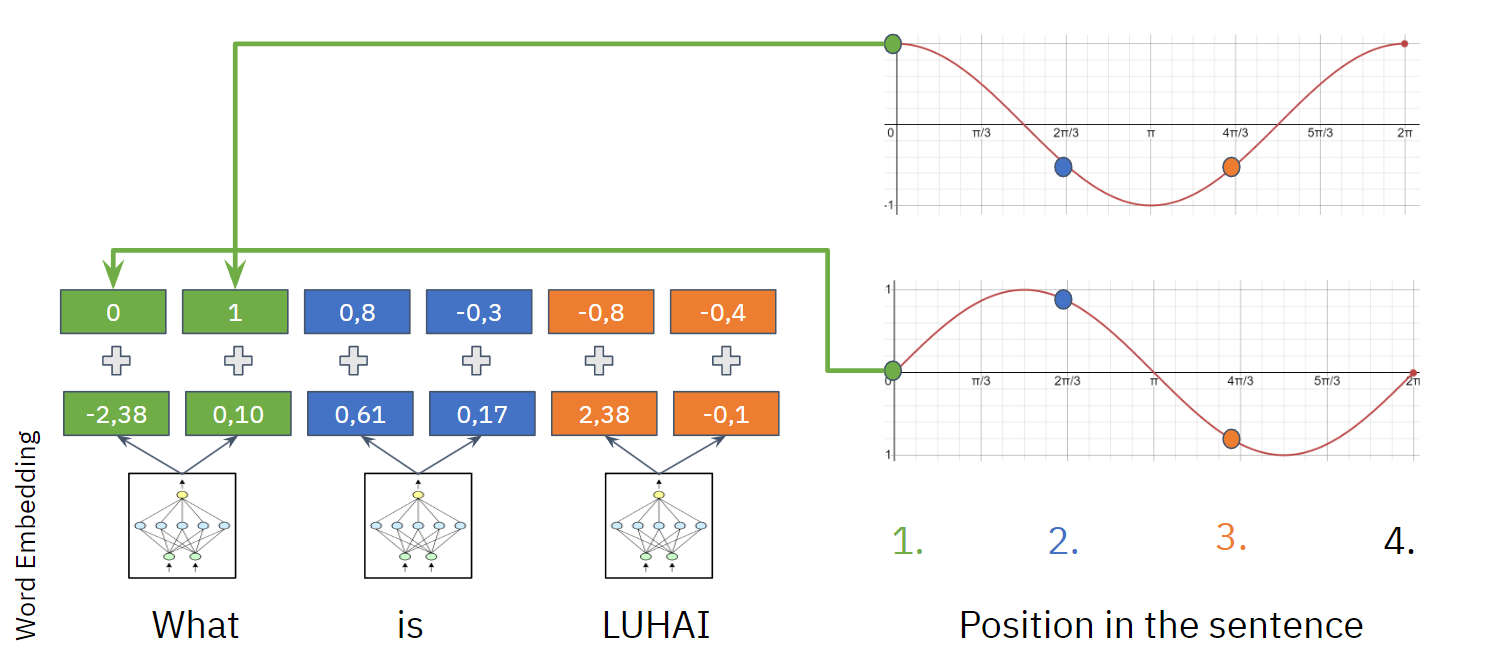
\includegraphics[width=0.9\linewidth]{075_deep_learning/figures/transformer4.png}
        
        \end{frame}

        %%%%%%%%%%%%%%%%%%%%%%%%%%%%%%%%%%%%%%%%%%%%%%%%%%%%%%%%%%%%%%
        \begin{frame}{Step2: Positional Encoding}

            \begin{itemize}
                \item Order matters!
            \end{itemize}

            \centering
            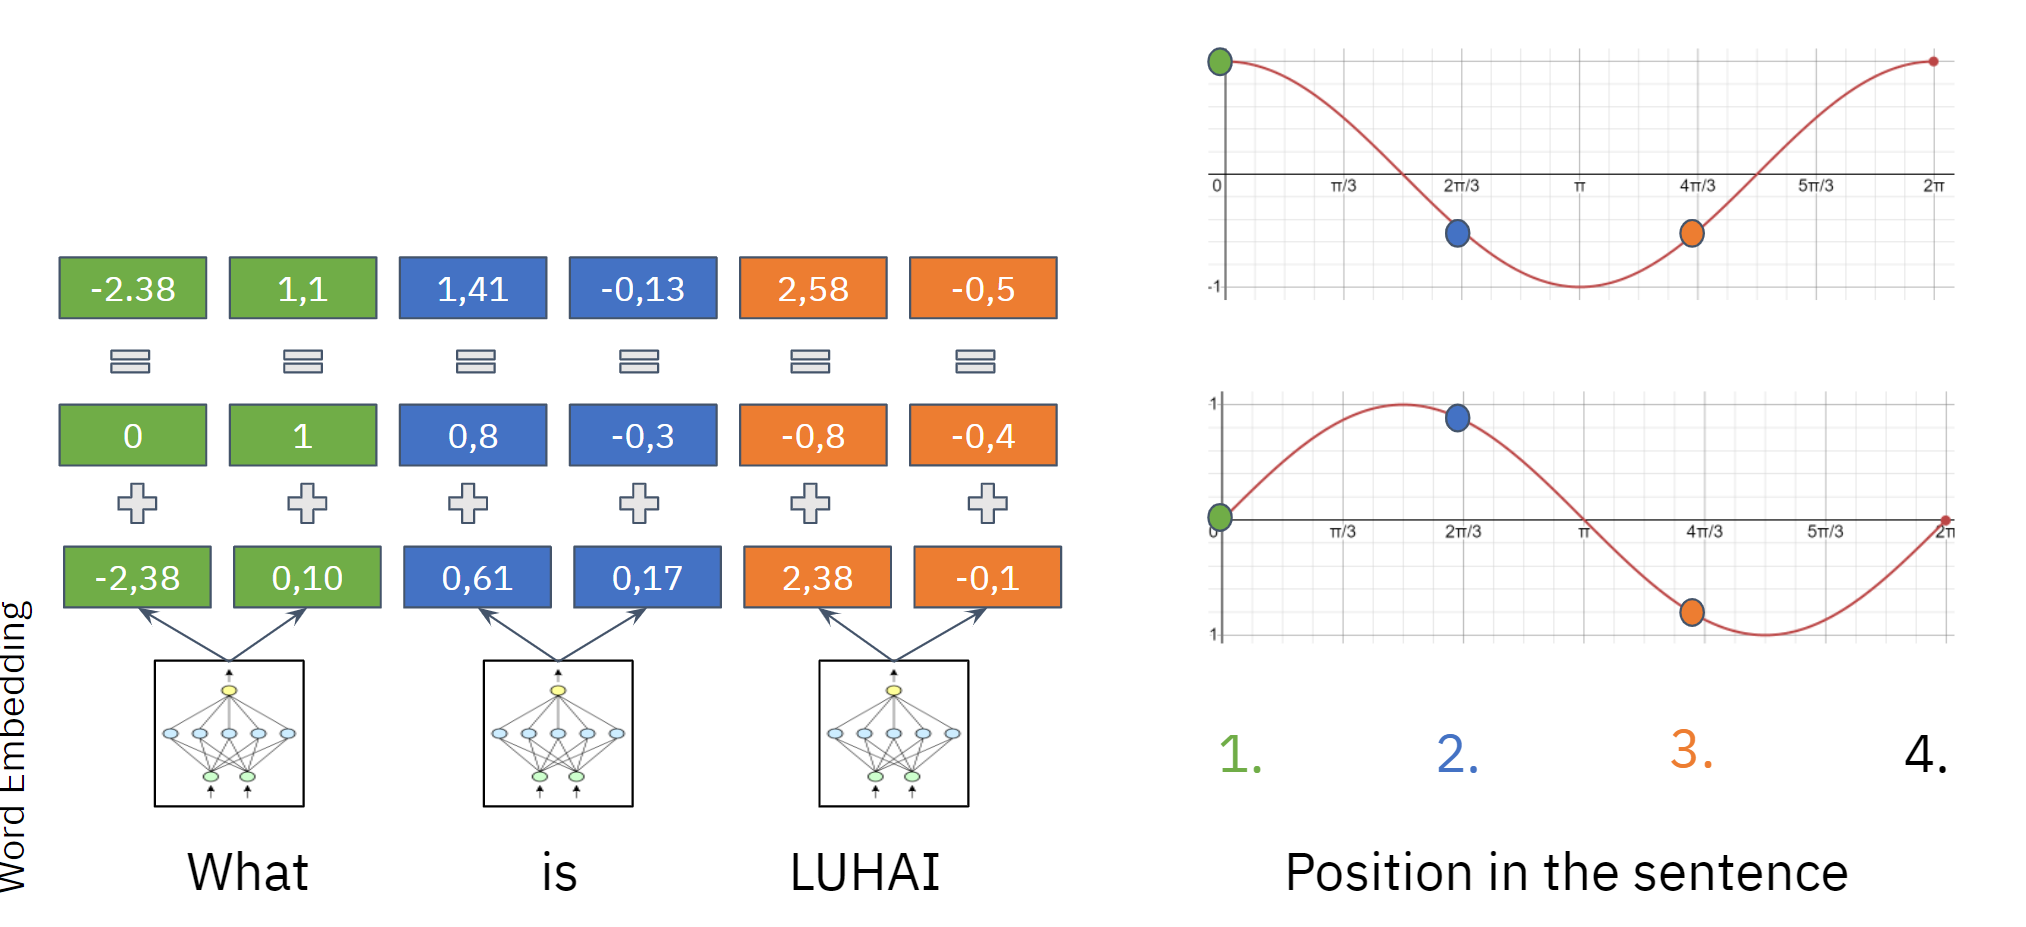
\includegraphics[width=0.9\linewidth]{075_deep_learning/figures/transformer5.png}
        
        \end{frame}

        %%%%%%%%%%%%%%%%%%%%%%%%%%%%%%%%%%%%%%%%%%%%%%%%%%%%%%%%%%%%%%
        \begin{frame}{Exemplary Chat III}

            \begin{itemize}
                \item Context matters!
            \end{itemize}

            \centering
            
\includegraphics[width=0.9\linewidth]{075_deep_learning/figures/transformer6.png}
        
        \end{frame}

        %%%%%%%%%%%%%%%%%%%%%%%%%%%%%%%%%%%%%%%%%%%%%%%%%%%%%%%%%%%%%%
        \begin{frame}{Self-Masked Attention: Query}

            \centering
            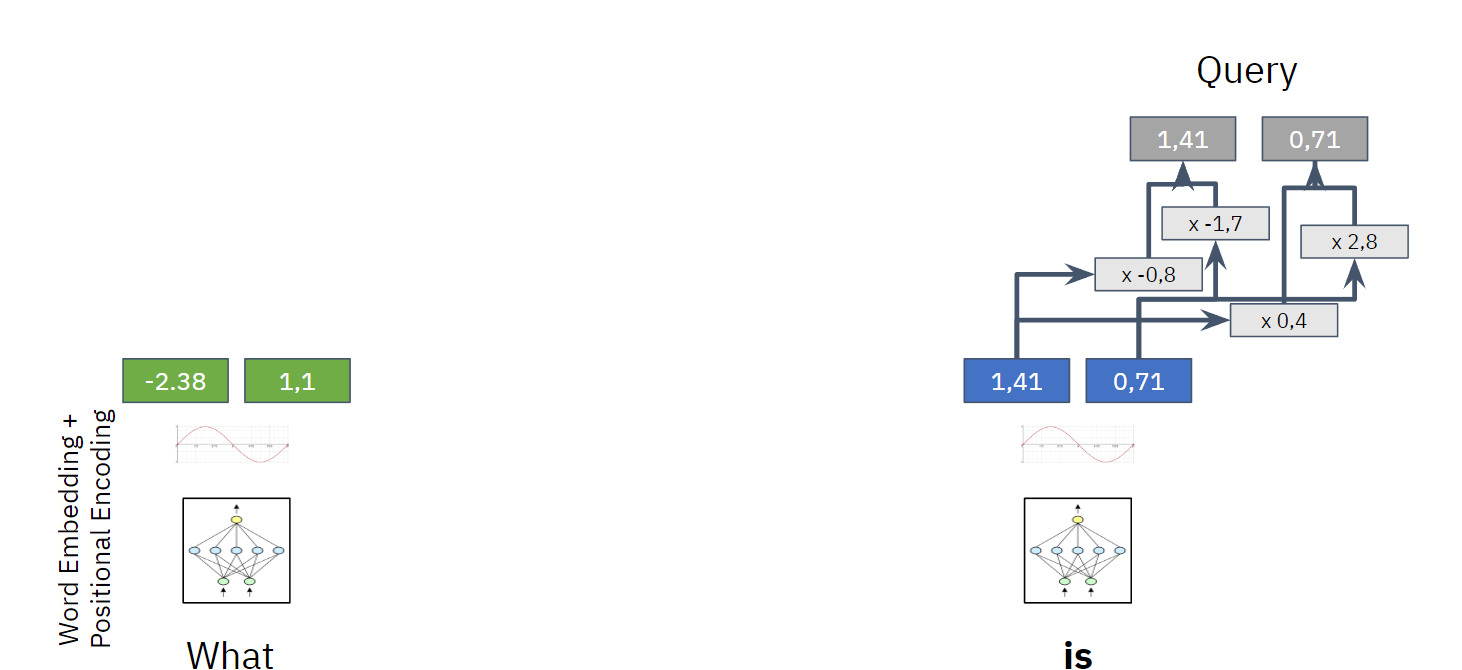
\includegraphics[width=0.9\linewidth]{075_deep_learning/figures/transformer7.png}
        
        \end{frame}

        %%%%%%%%%%%%%%%%%%%%%%%%%%%%%%%%%%%%%%%%%%%%%%%%%%%%%%%%%%%%%%
        \begin{frame}{Self-Masked Attention: Query}

            \centering
            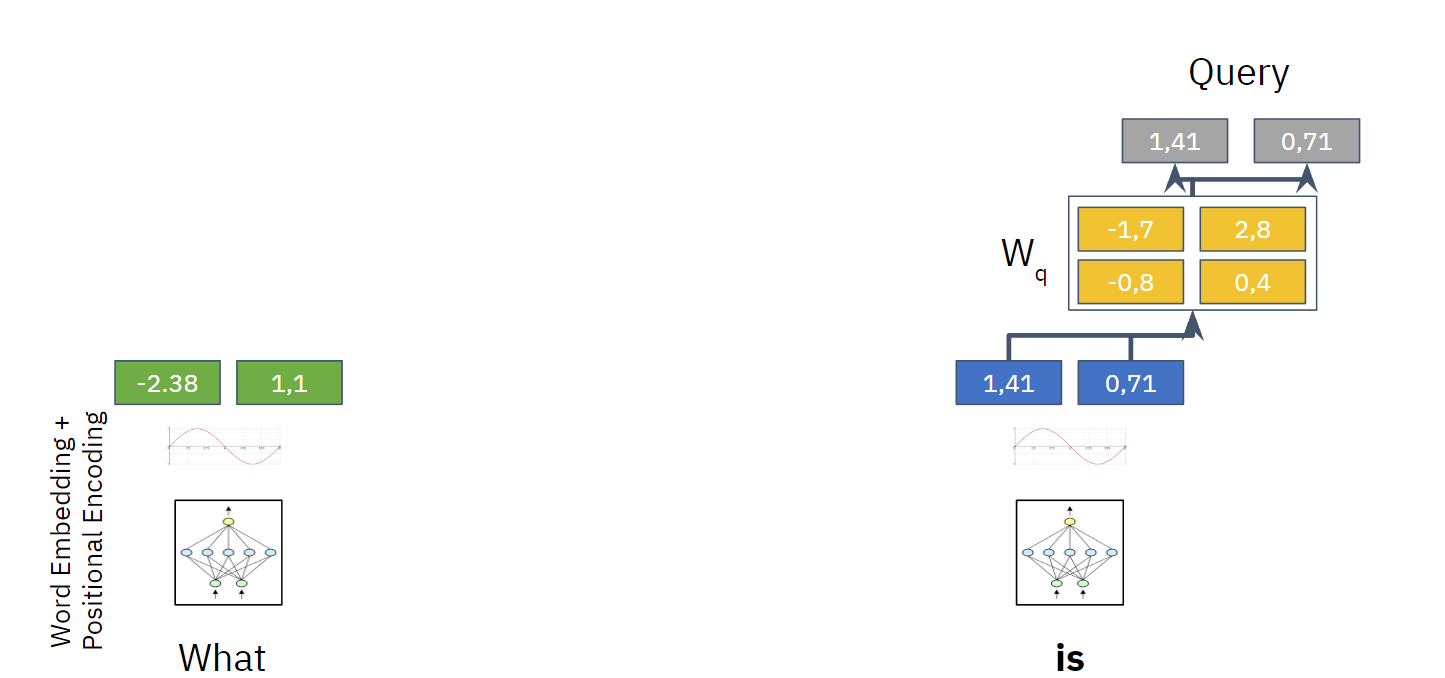
\includegraphics[width=0.9\linewidth]{075_deep_learning/figures/transformer8.png}
        
        \end{frame}

        %%%%%%%%%%%%%%%%%%%%%%%%%%%%%%%%%%%%%%%%%%%%%%%%%%%%%%%%%%%%%%
        \begin{frame}{Self-Masked Attention: Key}

            \centering
            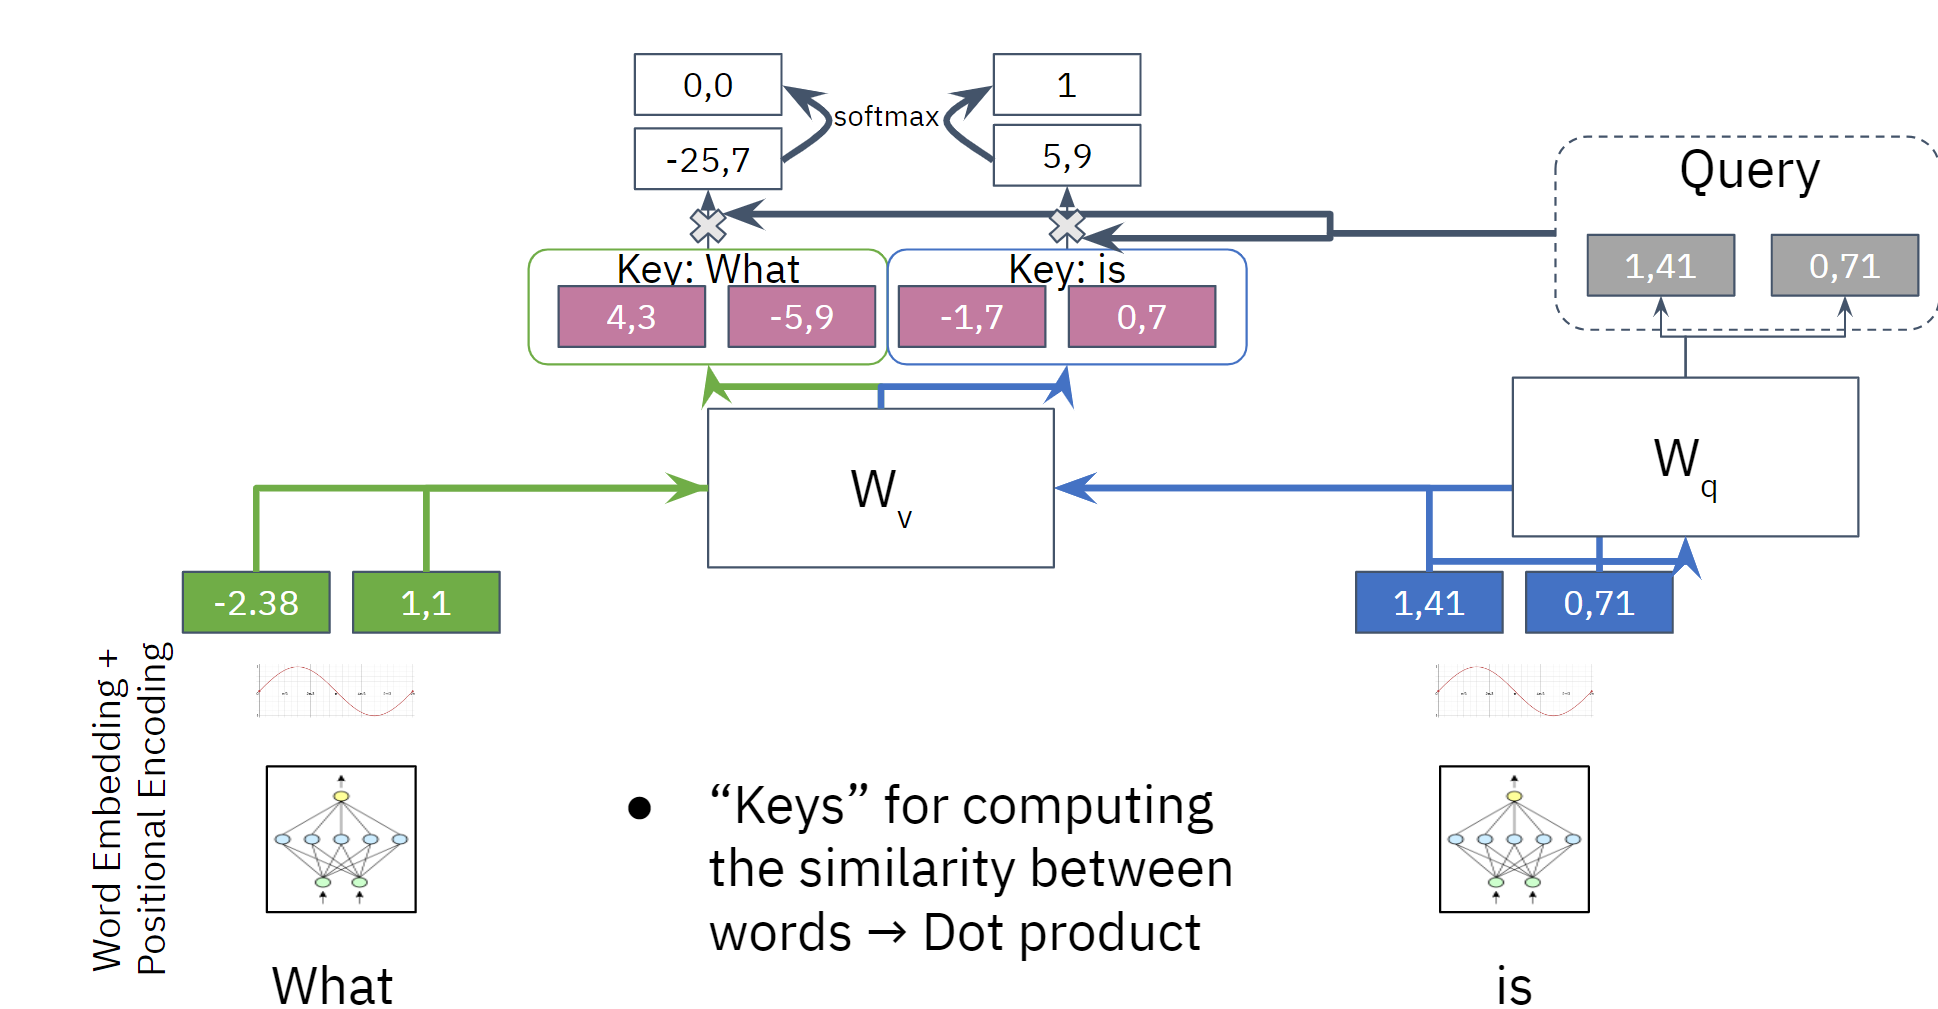
\includegraphics[width=0.9\linewidth]{075_deep_learning/figures/transformer9.png}
        \end{frame}
        %%%%%%%%%%%%%%%%%%%%%%%%%%%%%%%%%%%%%%%%%%%%%%%%%%%%%%%%%%%%%%
        \begin{frame}{Self-Masked Attention: Values}

            \centering
            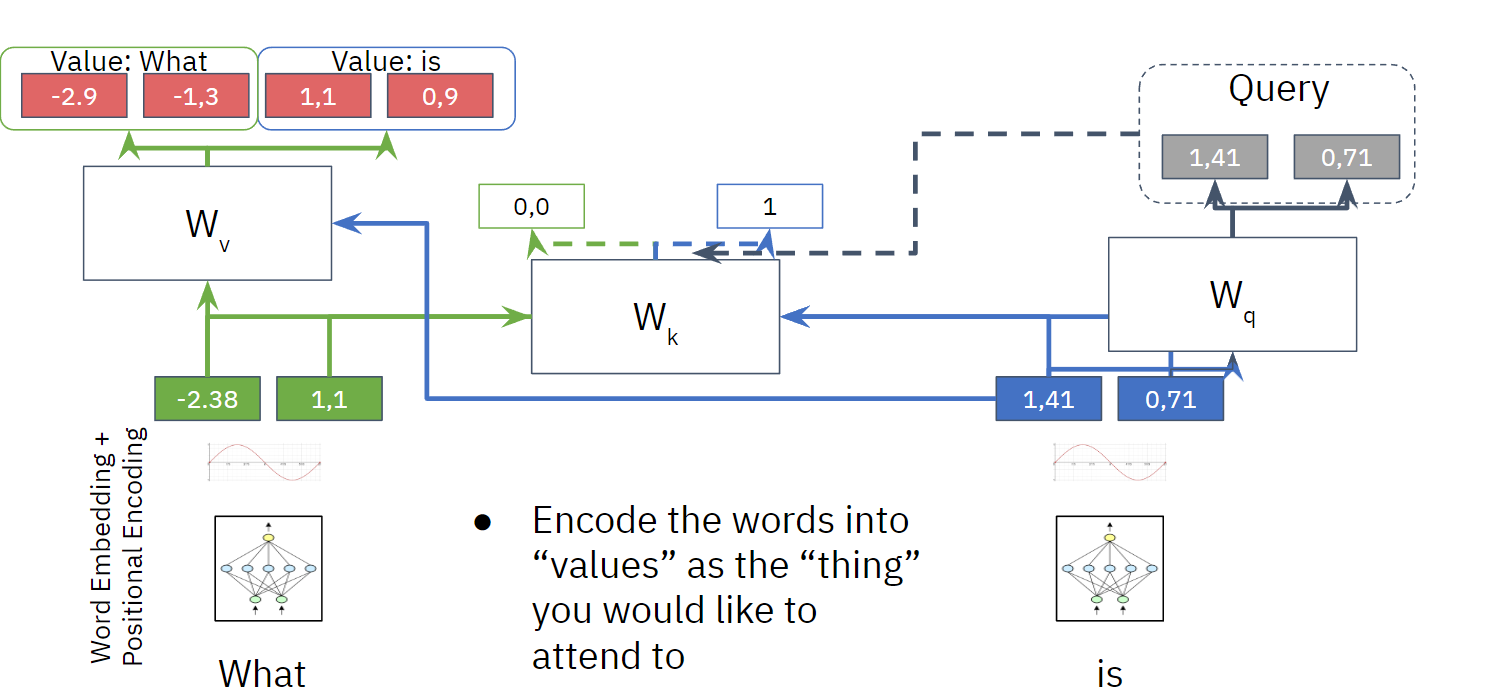
\includegraphics[width=0.9\linewidth]{075_deep_learning/figures/transformer10.png}
        
        \end{frame}

        %%%%%%%%%%%%%%%%%%%%%%%%%%%%%%%%%%%%%%%%%%%%%%%%%%%%%%%%%%%%%%
        \begin{frame}{Self-Masked Attention: Final}

            \centering
            \vspace{-1.2em}
            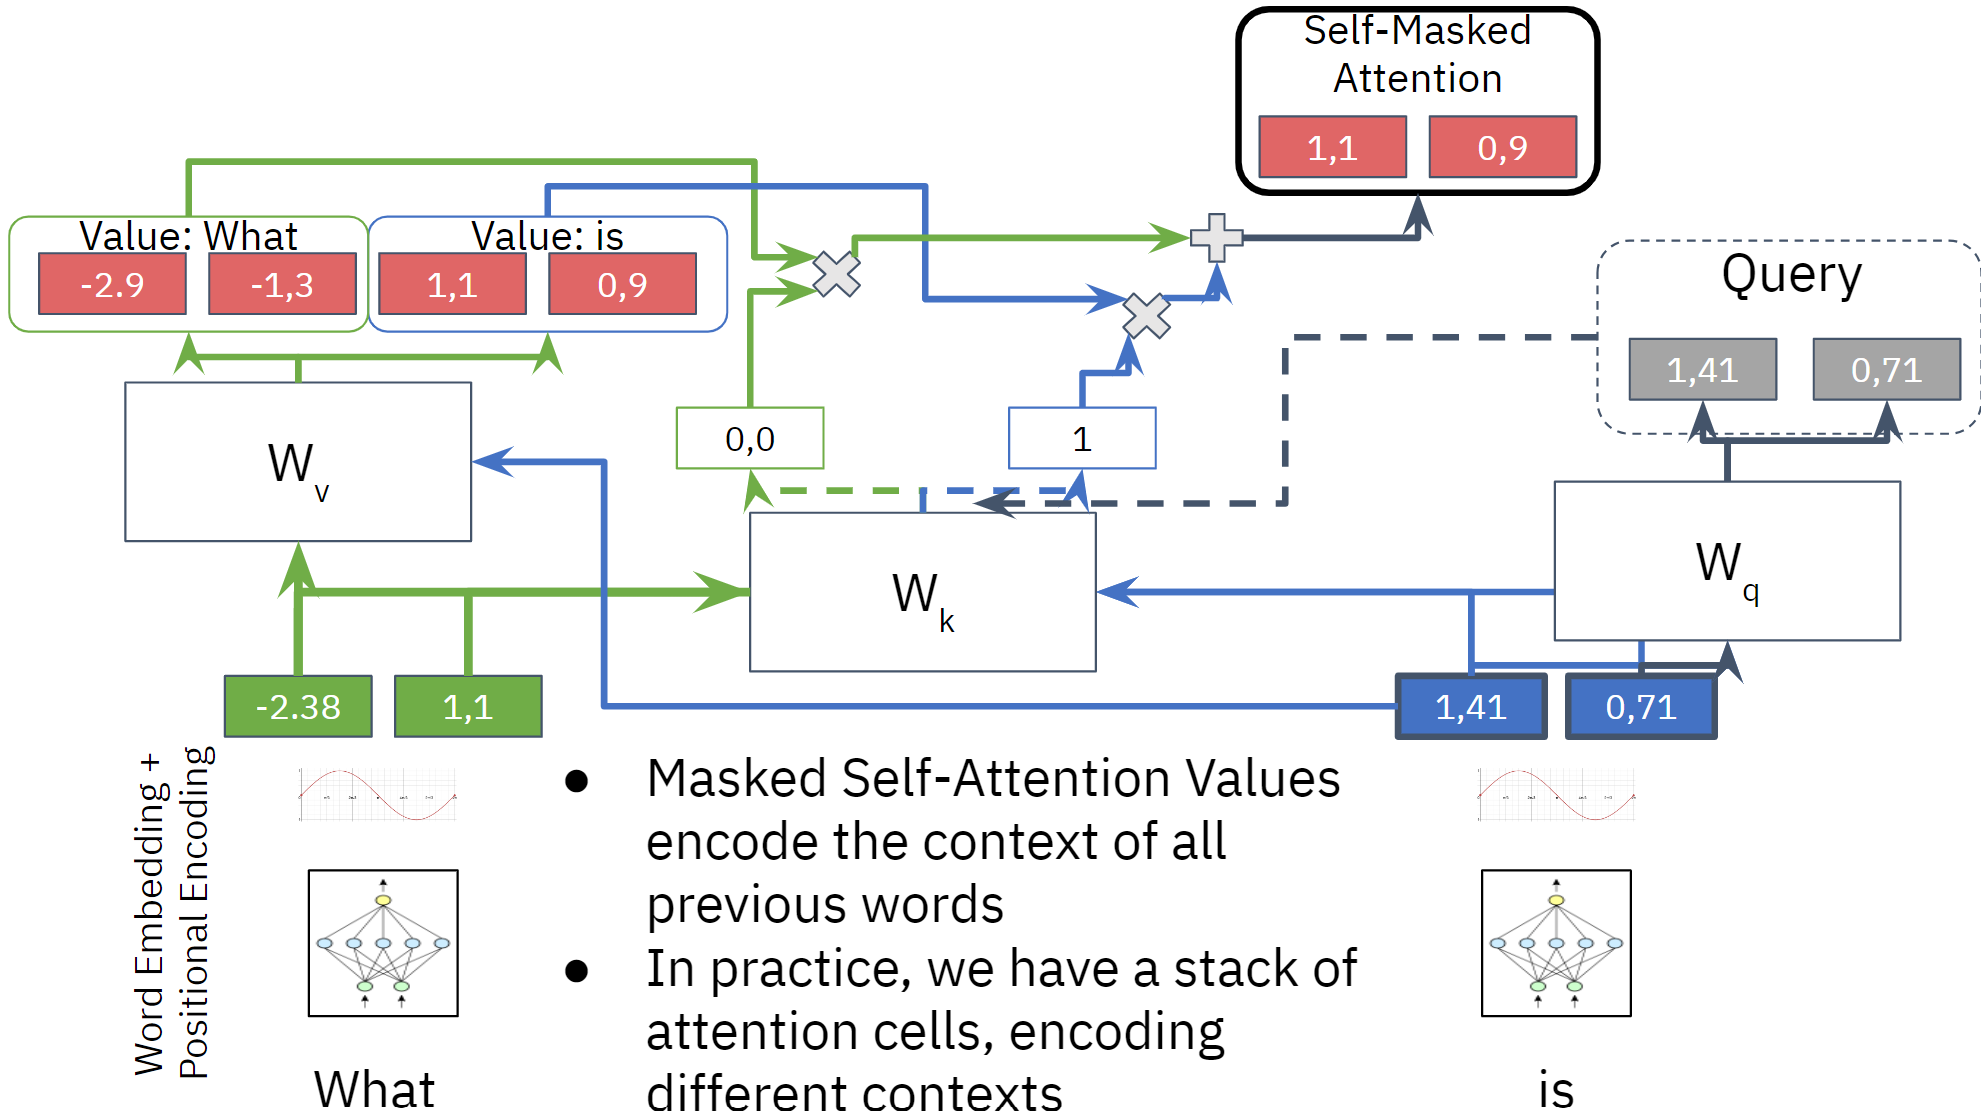
\includegraphics[width=0.9\linewidth]{075_deep_learning/figures/transformer11.png}
        
        \end{frame}

        %%%%%%%%%%%%%%%%%%%%%%%%%%%%%%%%%%%%%%%%%%%%%%%%%%%%%%%%%%%%%%
        \begin{frame}{Reverse Embedding}

            \centering
            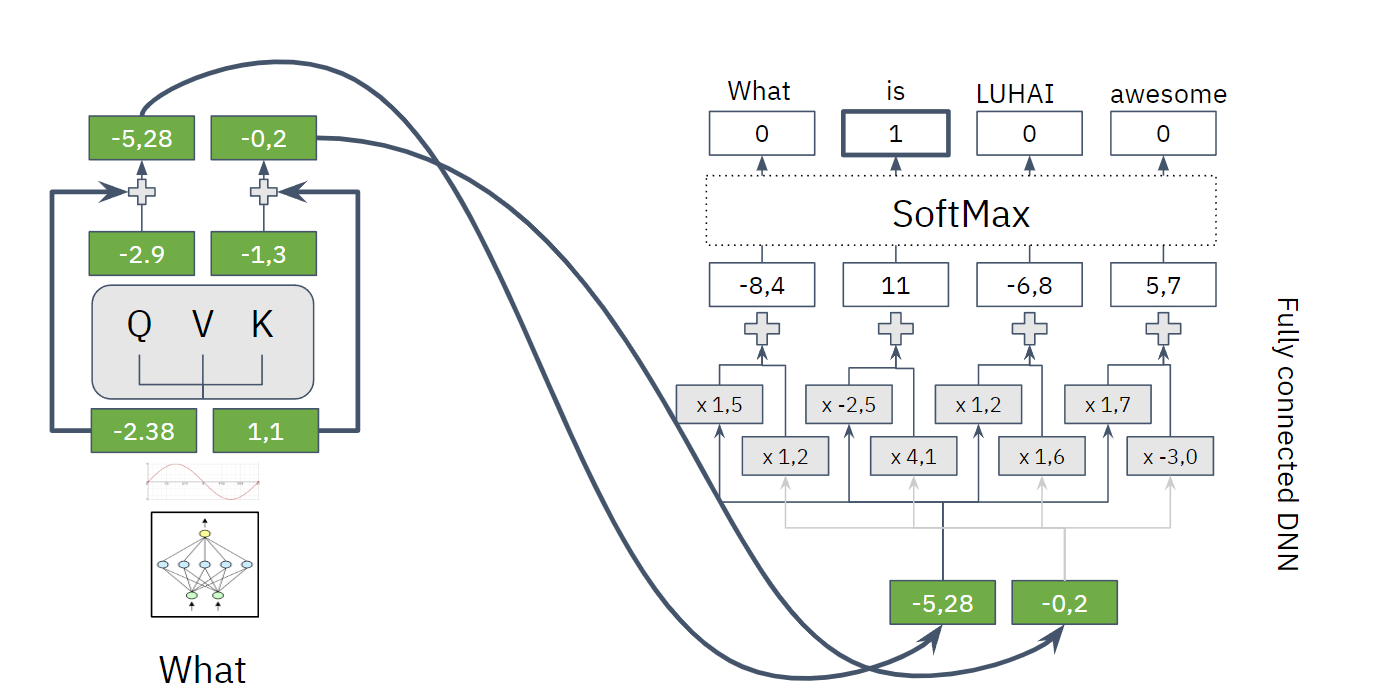
\includegraphics[width=0.9\linewidth]{075_deep_learning/figures/transformer12.png}
        
        \end{frame}

        %%%%%%%%%%%%%%%%%%%%%%%%%%%%%%%%%%%%%%%%%%%%%%%%%%%%%%%%%%%%%%
        \begin{frame}{Full Example}

            \centering
            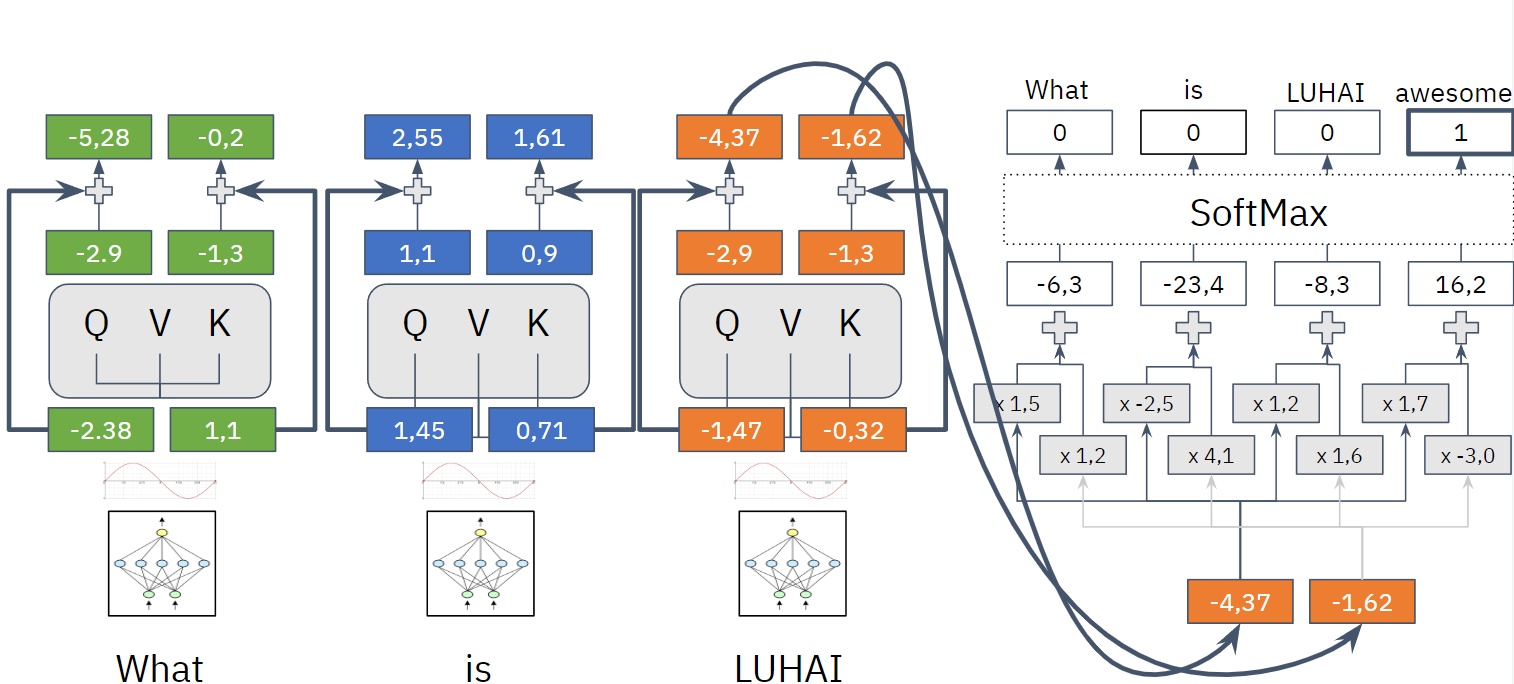
\includegraphics[width=0.9\linewidth]{075_deep_learning/figures/transformer13.png}
        
        \end{frame}

        %%%%%%%%%%%%%%%%%%%%%%%%%%%%%%%%%%%%%%%%%%%%%%%%%%%%%%%%%%%%%%
        \begin{frame}{Conclusion}

            \begin{itemize}
                \item Transformers are very powerful models 
                \begin{itemize}
                    \item nowadays they can deal with 10 thousands of tokens at once
                    \item but transformers often give special attention to the beginning and end of a sequence
                \end{itemize}
                \item There are quite some variants and further tricks for modern transformers, incl.
                \begin{itemize}
                    \item different positional encodings or not using it at all
                    \item order of the batch norm
                    \item different attention variants
                    \item use of encode-decoder vs only-decoder variants (e.g., GPT)
                \end{itemize}
            \end{itemize}
        
        \end{frame}
 	
\end{document}